\documentclass[conference]{IEEEtran}
\IEEEoverridecommandlockouts
% The preceding line is only needed to identify funding in the first footnote. If that is unneeded, please comment it out.
\usepackage{cite}
\usepackage{amsmath,amssymb,amsfonts}
\usepackage{algorithmic}
\usepackage{graphicx}
\usepackage{textcomp}
\usepackage{xcolor}
\usepackage{graphicx}
\def\BibTeX{{\rm B\kern-.05em{\sc i\kern-.025em b}\kern-.08em
    T\kern-.1667em\lower.7ex\hbox{E}\kern-.125emX}}
\begin{document}

\title{Untersuchung der Nachweisbarkeit des Akkommodation-Vergenzkonflikts in einem EEG in einer VR entspannungs Szene\\
\thanks{HFU Furtwangen}
}

\author{
	\IEEEauthorblockN{Nick Philipp Häcker}
	\IEEEauthorblockA{\textit{Fakultät Digitale Medien} \\
	\textit{Hochschule Furtwangen}\\
	Furtwangen, Deutschland \\
	haeckern@hs-furtwangen.de}
	
	\and
	\IEEEauthorblockN{Suzan Johannes}
	\IEEEauthorblockA{\textit{Fakultät Digitale Medien} \\
	\textit{Hochschule Furtwangen}\\
	Furtwangen, Deutschland \\
	s.johannes@hs-furtwangen.de}
	\and
	
	\IEEEauthorblockN{Patrick Kaserer}
	\IEEEauthorblockA{\textit{Fakultät Digitale Medien} \\
	\textit{Hochschule Furtwangen}\\
	Furtwangen, Deutschland \\
	patrick.kaserer@hs-furtwangen.de}
	\and
	
	\IEEEauthorblockN{Johann Schulenburg}
	\IEEEauthorblockA{\textit{Fakultät Digitale Medien} \\
	\textit{Hochschule Furtwangen}\\
	Furtwangen, Deutschland \\
	johann.schulenburg@hs-furtwangen.de}
	
	\and
	\IEEEauthorblockN{Lukas Willmann}
	\IEEEauthorblockA{\textit{Fakultät Digitale Medien} \\
	\textit{Hochschule Furtwangen}\\
	Furtwangen, Deutschland \\
	Lukas.willmann@hs-furtwangen.de}
}

\maketitle

\begin{abstract}
This document is a model and instructions for \LaTeX.
This and the IEEEtran.cls file define the components of your paper [title, text, heads, etc.]. *CRITICAL: Do Not Use Symbols, Special Characters, Footnotes, 
or Math in Paper Title or Abstract.
\end{abstract}

\begin{IEEEkeywords}
virtual reality, akkommodation-vergenz konflikt, elektroenzephalografie
\end{IEEEkeywords}

\section{Einleitung}
“Applications of Computer Science, including digital games, virtual reality, and augmented reality [...], have enormous potential for bringing about cultural change.” \cite{b3} Laut einer Prognose von ARtillery Intelligence soll zwischen 2021 bis 2026 der Umsatz von Virtual Reality weltweit von 8,3 auf 28,84 Milliarden US-Dollar steigen. \cite{b2} 
VR Brillen verwenden Stereoskopie, bei welcher jedem Auge leicht unterschiedliche Informationen durch eine horizontale Verschiebung der Bilder zugespielt werden, damit bei dem Nutzer eine 3D Wirkung der Darstellung entsteht. Durch die entstehenden Parallaxen kann die Szene den Eindruck erwecken, aus der Leinwand hervor zu stechen oder dahinter zu liegen.\cite{b4}
Die hier beschriebene Untersuchung konzentriert sich auf den Accommodation Vergenz Konflikt. Dieser tritt gerade in der modernen VR Technologie auf, da durch die Linsen der VR Brille die Bildebene in eine weite Entfernung projiziert wird und die Objekte in VR durch die Interaktion in greifbarer Nähe sind.
“In order to see one object, the eyeballs need to rotate accordingly. This mechanism is called the “vergence”. In a natural situation, as an object is moving closer or further, vergence matches another physiological phenomena: “accommodation”. It enables the object’s image to remain clear on the retina. It is caused by a deformation of the crystalline lens, which focuses light beams the same way camera lenses do.”\cite{b1}

Besonders interessante Hirnregionen bezüglich der Okulomotorik sind hierbei unter anderem das  Mittelhirn aus welchem drei Hirnnerven zu den Augen verlaufen wobei der N. oculomotorius unter anderem auch für die Akkommodation des Auges zuständig ist \cite{b6}. Hierbei ist es vor allem anspruchsvoll erkennbar zu machen ob die gemessenen Werte des EEGs wirklich durch den Akkommodation-Vergenzkonflikt kommen, da beim Sehvorgang diverse Regionen des Gehirns angesprochen werden wie die primäre Sehrinde im hinteren Hauptlappen der Großhirnrinde, der Scheitellappen unter anderem zur Erkennung wo sich etwas befindet und der Schläfenlappen zur Objekterkennung etc. \cite{b8}. Schlussendlich könnte evtl. der primär sensorische Kortex mit den Bereichen die Wilder Penfield ermittelt hat durch starke Werte vermitteln ob sich ein Einfluss des Akkommodation-Vergenzkonfliktes im EEG nachweisen lässt \cite{b7}.

Durch den Versuch soll aufgezeigt werden, ob mögliche Probleme in Anwendungen, welche in dem kritischen Bereich des Akkommodation-Vergenz Konflikt arbeiten, durch das EEG nachweisbar sind oder nicht. Somit kann sich zukünftige Forschung ebenfalls diesem Bereich widmen.

\section{Related Work}
\subsection{Assessing the zone of comfort in stereoscopic displays using EEG}
Im Rahmen des Papers "Assessing the zone of comfort in stereoscopic displays using EEG" \cite{b1} wurde untersucht, wie sich der Akkommodations-Vergenz-Konflikt bei stereoskopischen Anzeigen auf die EEG-Aktivität auswirkt. Das Ziel war es, ein adaptives System zu entwickeln, das mithilfe von leichtgewichtigen EEG-Geräten die Anzeige individuell auf jeden Betrachter kalibrieren kann, um unangenehme Erfahrungen zu vermeiden.\\ 
Eine Pilotstudie wurde durchgeführt, bei der kurze Betrachtungssequenzen verwendet wurden, um Ergebnisse innerhalb eines kurzen Zeitraums vor der Gewöhnung bei den Probanden zu erzielen. Der Versuchsaufbau bestand darin, dass der Proband einen Meter vor einen Bildschirm gesetzt wurde. Dieser zeigte zuerst eine Szene von 2-5 Sekunden in der ein Würfel in Null-Parallaxe auf dem Bildschirm dargestellt wurde. Darauf wurde er zufällig in eine von 9 Positionen 5 Sekunden lang vor oder hinter den Bildschirm stereoskopisch dargestellt. Diese Positionen reichten von 0.212 m vom Probanden entfernt bis 3,046 m vom Probanden entfernt. Sie wurden in Positionen eingeteilt die als komfortabel (C) oder unkomfortabel (NC) klassifiziert wurden. Nach den 5 Sekunden musste der Proband angeben ob der Würfel vor oder hinter dem Bildschirm lag. Dieser Versuch wurde sowohl nur mit Fragebogen als auch mit einer EEG Messung und einem Fragebogen durchgeführt. Bei der EEG Messung gab es 3 Probanden.\\ 
In der Analyse der ereignisbezogenen Potenziale (ERP) ergaben sich Unterschiede zwischen den Bedingungen C und NC. In der NC-Bedingung war die positive Komponente im ERP verzögert, während die negative Komponente in der C-Bedingung eine höhere Amplitude aufwies. Die Untersuchung der Frequenzbänder (ERSP) zeigte ebenfalls Unterschiede zwischen den Bedingungen C und NC. In der NC-Bedingung wurde eine Abnahme der Aktivität im Alpha-Band (10-14 Hz) festgestellt, während eine Zunahme der Aktivität im Theta-Band (4-7 Hz) und Beta-Band (15-25 Hz) im Vergleich zur C-Bedingung beobachtet wurde. Die Probanden schnitten in der unkomfortablen Bedingung besser bei der Tiefenwahrnehmung ab. Die Ergebnisse des Umfragebogens ergaben dabei, dass klares Unwohlsein durch die visuelle Darstellung ausgelöst wurde. Es wurden Widersprüche zu früheren Studien festgestellt, die Stereoskopie mit 2D-Bildern verglichen haben. Es wurden Verbesserungen vorgeschlagen, wie die Messung des Pupillenabstands und die Verwendung fortschrittlicherer Technologien wie VR-Brillen. Die Autoren vermuten, dass die EEG-Messung nicht nur zur Optimierung der Stereoskopie dienen kann, sondern auch zur Entwicklung von Leitlinien für eine verbesserte Technologie.\\
In unserem Versuch können wir unsere EEG-Ergebnisse mit den Ergebnissen dieses Papers bezüglich der EEG-Ergebnisse vergleichen. Unterschiede welche hierbei jedoch hervorzuheben sind dabei, dass die 3D-Szene deutlich komplexer ist als der Aufbau in diesem Paper. Ebenfalls muss man die Anzahl der Versuchspersonen hervorheben und dass in unserem Versuch eine konstante Veränderung der Position des Würfels durchgeführt wird und nicht zu jeder Position der Sehkomfort abgefragt wurde. Bezüglich des technischen Aufbaus muss man berücksichtigen, dass in unserem Versuch beim Einrichten der VR-Brille die IPD der Probanden beachtet wurde und mit der VR-Brille ein deutlich immersiveres Medium verwendet wurde als ein 3D Bildschirm.


\subsection{Study of Electroencephalography-based Objective Stereoscopic Visual Fatigue Evaluation}
In dem Paper "Study of Electroencephalography-based Objective Stereoscopic Visual Fatigue Evaluation" \cite{b5} wird der Bezug zwischen visueller Ermüdung durch den Akkommodation-Vergenz Konflikt bei 3D-Displays hergestellt mittels einer EEG-Messung.\\
Das Experiment wurde an 11 Studenten durchgeführt. Hierbei sollten die Probanden auf einem Random Dot Stereogram feststellen in welche Richtung ein abgebildeter Pfeil zeigt. Es gab 5 Minuten Übungszeit und darauf 7-mal 10 Minuten die Durchführung des Tests.\\
Die Forscher konnten einen stärkeren Anstieg der Alpha-Wellen im Frontalen Bereich des Gehirns feststellen über die Dauer des Experiments. Die Aktivität der Beta-Wellen stieg auch an, jedoch nicht so stark wie die der Alpha Wellen. Die Forscher stellten in ihrer Forschung fest, dass die Art der Aufgabe auch Einfluss auf die Aktivitäten der Wellen genommen haben kann. Sie schlussfolgern, dass ihr Ergebnis der erhöhten Alpha-Wellen Aktivität gerade im Frontallappen ein Anzeichen für visuelle Ermüdung sein kann.\\
Auch hier können die Ergebnisse des EEGs mit unseren Ergebnissen verglichen werden. Aufgrund der Beschreibung des Versuchsaufbaus wird nicht klar wie stark in dem Versuch der Akkommodation-Vergenz Konflikt erzeugt wurde. Es ist außerdem zu beachten, dass ein Random Dot Stereogram auf einem 3D-Display sehr abweichende Ergebnisse liefern kann im Vergleich zu einer Komplexen 3D Szene auf einem VR-Headset.
 

\section{Methodik}
\subsection{Material}
Als VR-Brille wurde eine Vive Pro \cite{b11} verwendet. Die EEG Messung wurde mit dem DSI-24 von Neurospec durchgeführt \cite{b9}. Einem Dry Sensor Interface. Zur Verwaltung der Antworten im SSQ und der allgemeinen Daten wurden die Fragebögen mit Google-Forms erstellt. Aus Datenschutzgründen wurden zur Zuordnung der Daten anonyme Codes verwendet und keine personalisierten Daten der Probanden online abgespeichert. Zur Auswertung der EEG Daten wurde die Software "Besa Research" von BESA verwendet \cite{b10}. Die verwendete Entspannungszene in welcher der Proband sich während dem Test befindet wurde von einer vorherigen Forschungsgruppe in Unity entwickelt. Diese konnte Ergebnisse erzielen welche auf einen positiven Effekt auf die Entspannung der Nutzer schließen lässt. Anpassungen für dieses Experiment und die Ausführung des Experiments wurden ebenfalls in Unity durchgeführt.

\subsection{Versuchsdurchführung}
Das Experiment wurde in den Räumlichkeiten der Hochschule Furtwangen durchgeführt. Vor der Durchführung des Tests wurden die Versuchspersonen auf bekannte Sehschwächen, Epilepsie oder vorhandene partielle Blindheit befragt. Nach der Zustimmung der Einverständniserklärung bezüglich Datenverarbeitung und Risiken wurde ein Random-Dot Test zur Erfassung des möglichen Tiefensehens durchgeführt und die IPD vermessen. Danach füllte der Proband einen Pre-Simulator-Sickness-Questionaire aus. Der Proband wurde nach dem SSQ auf einen Liegestuhl gebeten. Hier wurde die VR-Brille passend zur gemessenen IPD angelegt und das EEG aufgesetzt. Der Proband wurde aufgeklärt, dass er während dem Test starkes Zwinkern, bewusste Kopfbewegungen oder auf die Zähne beißen vermeiden sollte, da dies alles Einfluss auf die EEG Messdaten hat.\\
Der Proband bekam nachdem alle Geräte angelegt und kalibriert waren ein Entspannungsszene vorgespielt. In dieser Szene befindet sich ein Würfel welcher einen grünen Punkt als Markierung auf seiner Oberfläche besitzt. Die Markierung soll zur leichteren Fokussierung des Würfels dienen. Nachdem der Proband mit einem Handzeichen signalisiert hatte, dass er sich in der Szene wohl fühlt kam der Würfel langsam auf ihn zu. Hierbei sollte der Proband durchgängig den Würfel fokussieren. Der Würfel legt hierbei innerhalb von 4 Minuten einen Weg von ca. 13 Meter bis auf 13 Zentimeter Entfernung zum Probanden in VR zurück. Sobald der Würfel bei 13 Zentimeter angekommen ist verweilte er dort 10 Sekunden. Danach füllte der Proband den Post-Simulator-Sickness-Questionaire aus.\\
Der Stimuli des Tests ist der Würfel, welcher sich dem Probanden durchgehend in den 4 Minuten in einer konstanten Geschwindigkeit nähert. Um das Erkennen der genauen Entfernung des Würfels für den Probanden zu verhindern wurde der Würfel in seiner Skalierung verhältnismäßig zur Entfernung zum Probanden kleiner Skaliert (…f*Scale/distance… richtige Formel einfügen). Durch die Entfernung dieser monokularen Tiefeninformation soll das Annähern des Würfels eine mögliche bedrohliche Wirkung auf den Probanden verringern. In der Szene wurde ein Bereich gewählt in welchem möglichst wenig Bäume  vorhanden sind, damit es beim Probanden nicht zu Problemen der Fixationsdisparitäten kommt.\\
Die Durchführung des Experiments betrug ca. 25-50 Minuten. 7-10 Minuten benötigte die Einführung und die Fragebögen, 5 Minuten die Zeit in VR und ca. 10-35 Minuten das Anlegen und Kalibrieren des EEGs. 

\subsection{Datenerhebung und Verarbeitung}
Die Daten welche mit Google Forms erhoben wurden, konnten als csv-Dateien heruntergeladen werden. Diese Daten wurden in Excel verarbeitet. Die demografischen Daten wurden als Kreisdiagramme (vgl. Fig. 2) und Boxplots dargestellt (vgl. Fig 1).
Die Ergebnisse des SSQ Fragebogen wurden im Vorher-Nachher Vergleich als Boxplots gegenüber gestellt. (vgl. Fig 3).\\
Um eine mögliche Signifikanz der Vorher- und Nachher Ergebnisse der SSQ Ergebnisse zu ermitteln wurde in Excel ein einseitiger t-Test durchgeführt.\\ 
!! Nick hier seinen Teil !!

\section{Ergebnisse}
Durch die t-Test Analyse konnten keine signifikanten Ergebnisse bei allen Indikatoren des SSQ-Tests ermittelt werden. Die Nullhypothese, dass die Durchführung in der VR-Szene des Tests zu Simulator-Sickness führt musste nicht verworfen werden. Bei einem Alpha = 0.05 wurden die geringsten Werte bei Schwitzen (p = 0,052) und Erhöhter Speichelfluss (p = 0,082) festgestellt werden.\\
\begin{figure}[ht]
	\centering
	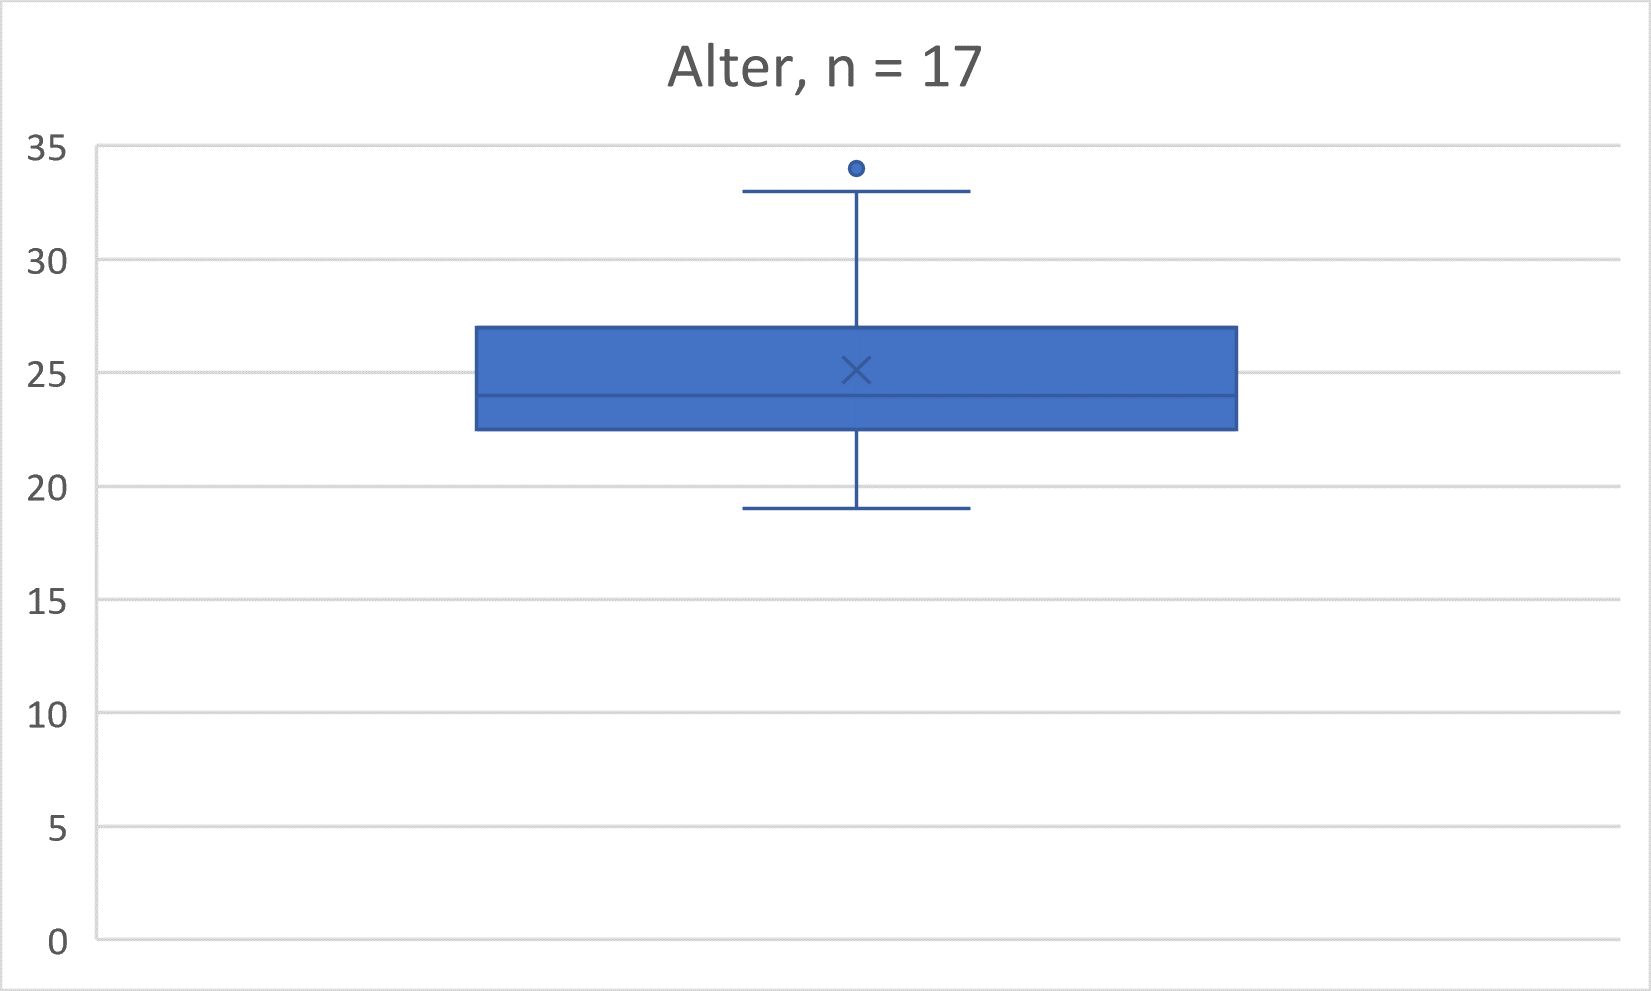
\includegraphics[width=0.2\textwidth]{assets/alter.png} \hspace{-5pt}
	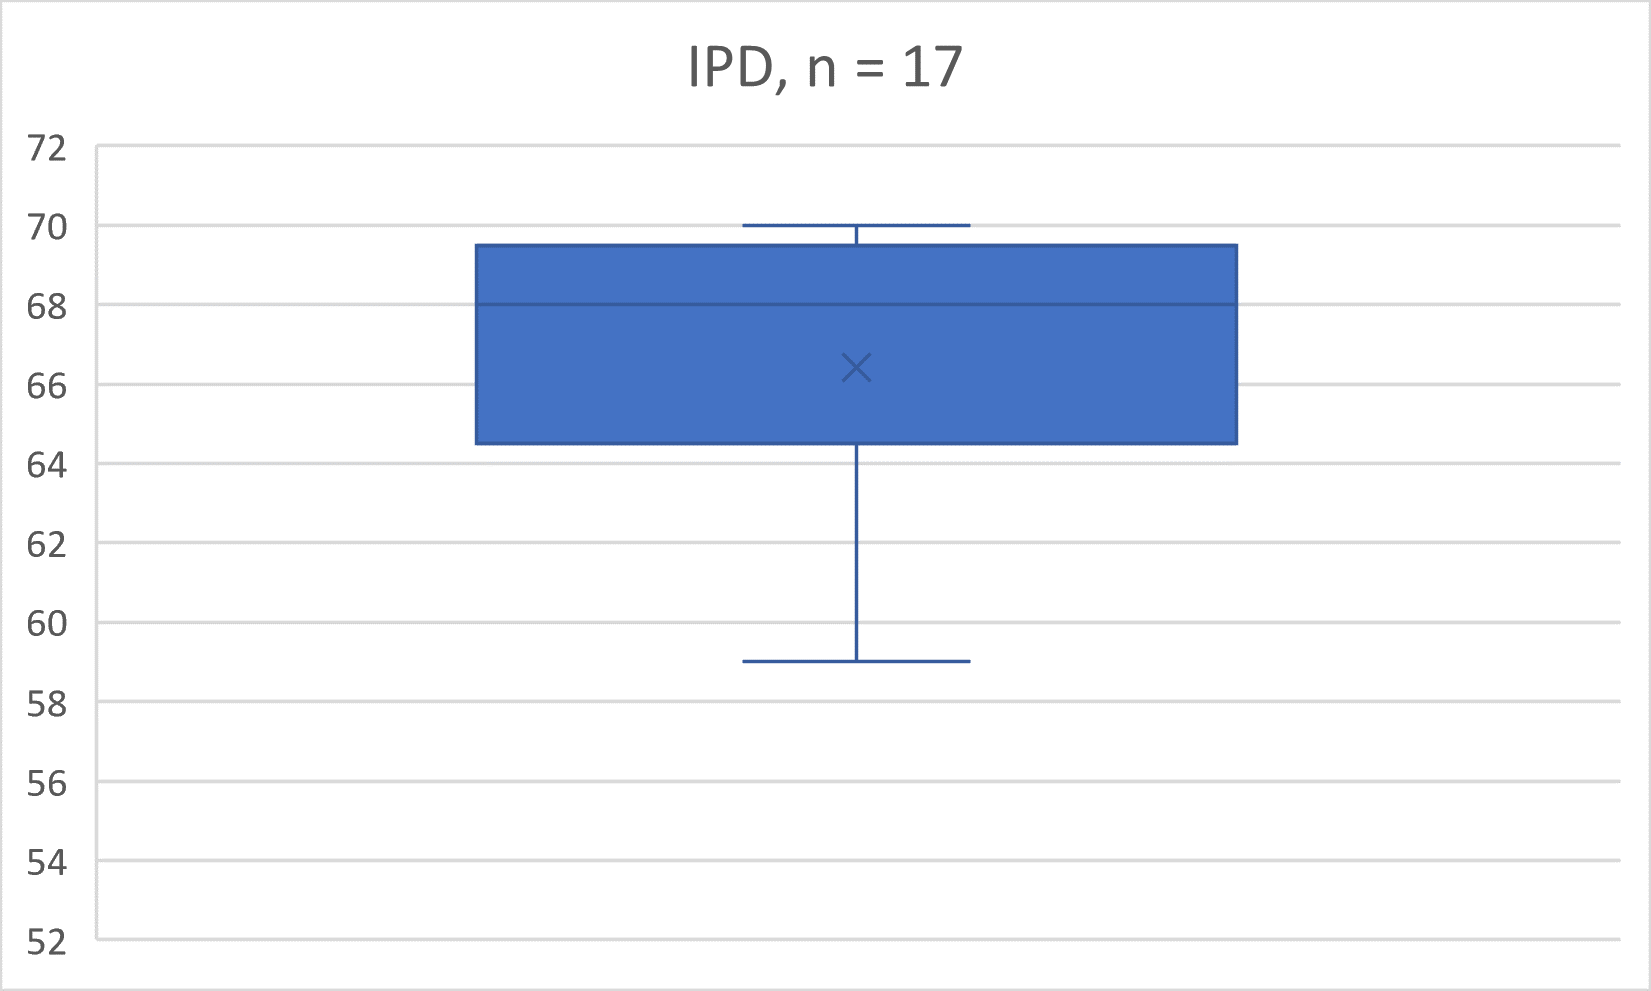
\includegraphics[width=0.2\textwidth]{assets/ipd.png} \\
	\vspace{2pt}
	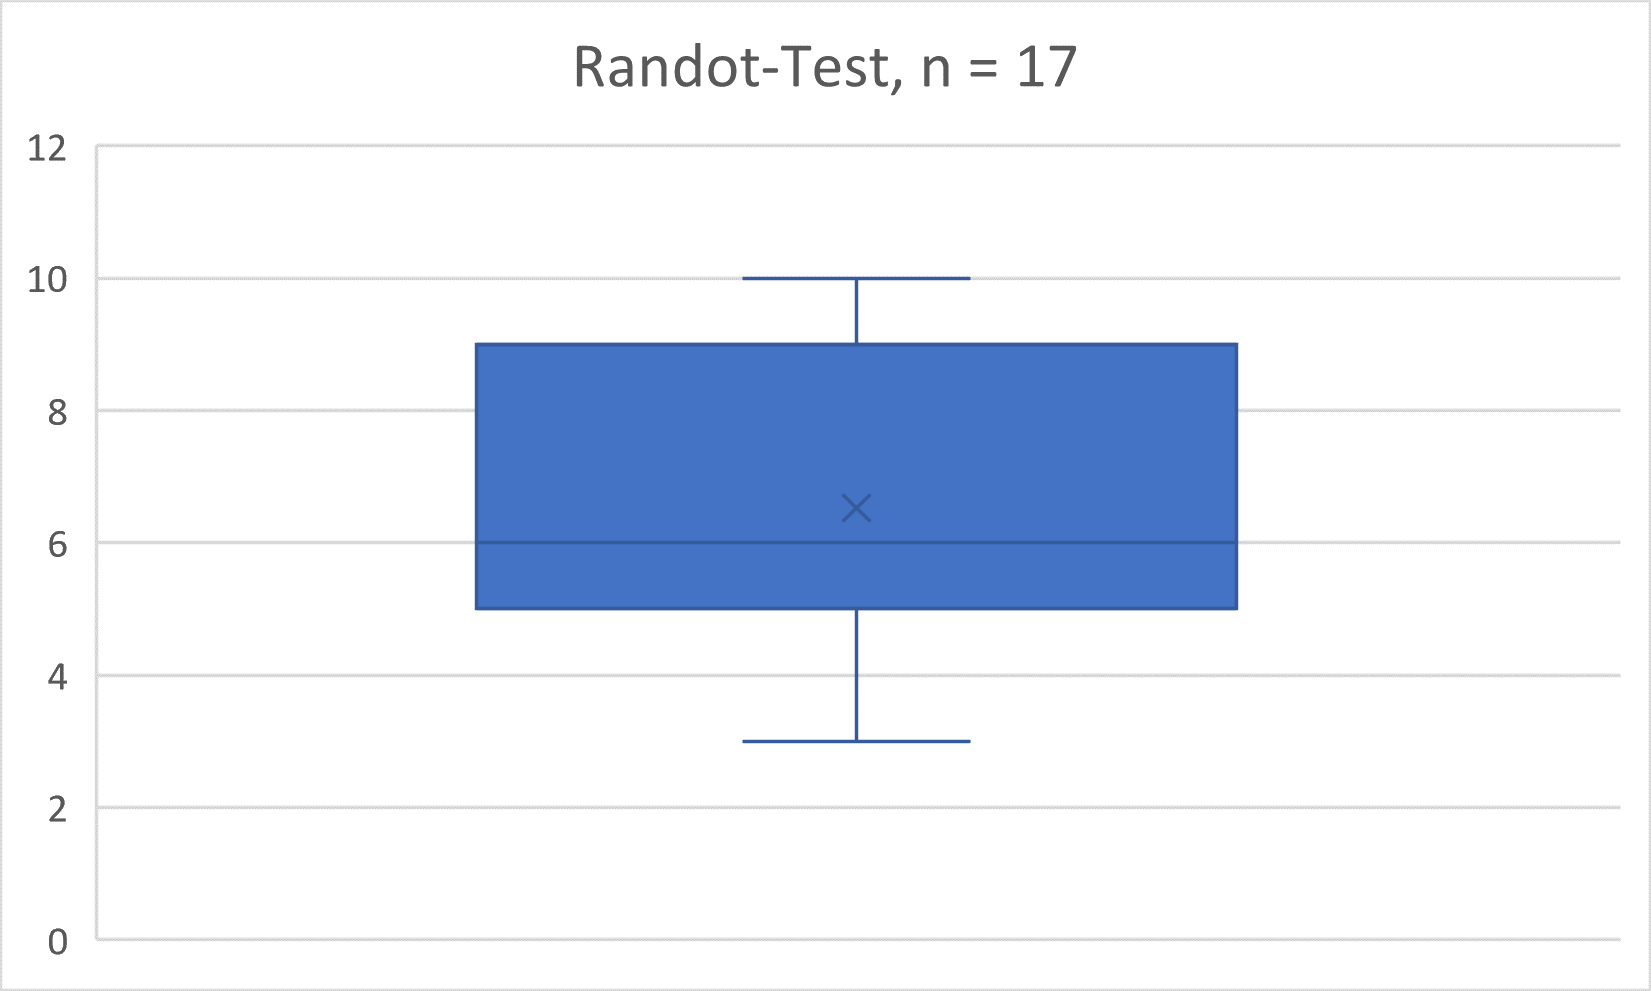
\includegraphics[width=0.2\textwidth]{assets/randot.png} \hspace{-5pt}
	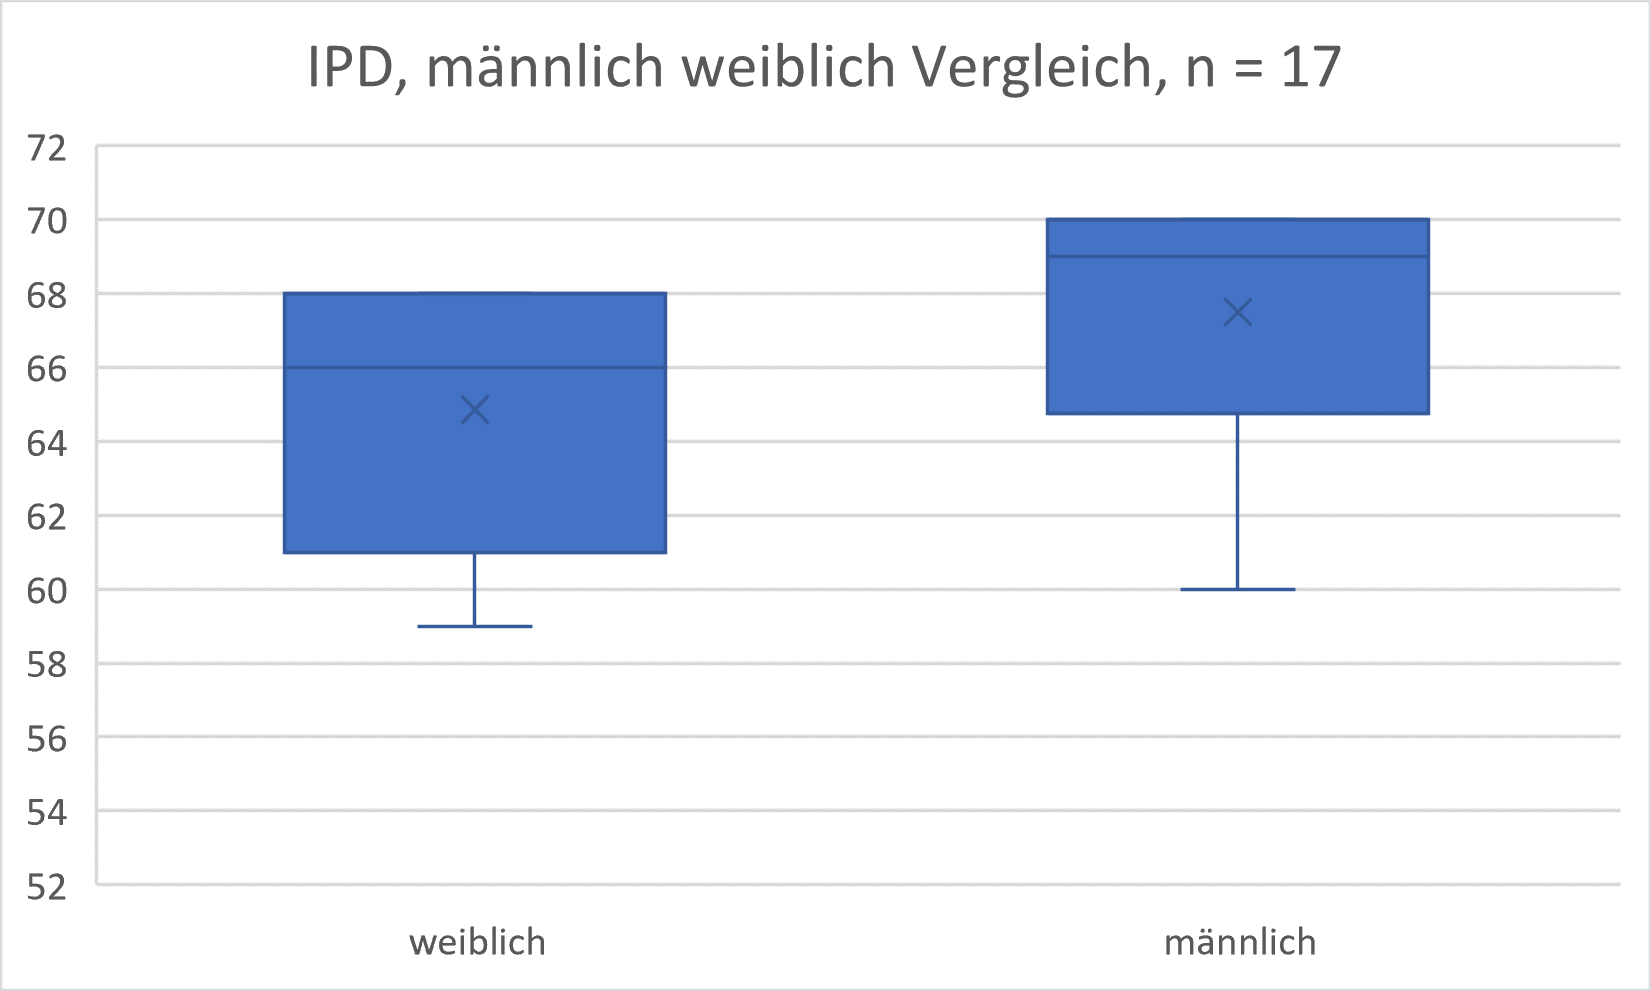
\includegraphics[width=0.2\textwidth]{assets/ipd_mvw.png}\\
	\caption{Demografische Daten}
	\label{fig:Demografische Daten}
\end{figure}
Lorem ipsum dolor sit amet, consetetur sadipscing elitr, sed diam nonumy eirmod tempor invidunt ut labore et dolore magna aliquyam erat, sed diam voluptua. At vero eos et accusam et justo duo dolores et ea rebum. Stet clita kasd gubergren, no sea takimata sanctus est Lorem ipsum dolor sit amet. Lorem ipsum dolor sit amet, consetetur sadipscing elitr, sed diam nonumy eirmod tempor invidunt ut labore et dolore magna aliquyam erat, sed diam voluptua. At vero eos et accusam et justo duo dolores et ea rebum. Stet clita kasd gubergren, no sea takimata sanctus est Lorem ipsum dolor sit amet.

\begin{figure}[ht]
	\centering
	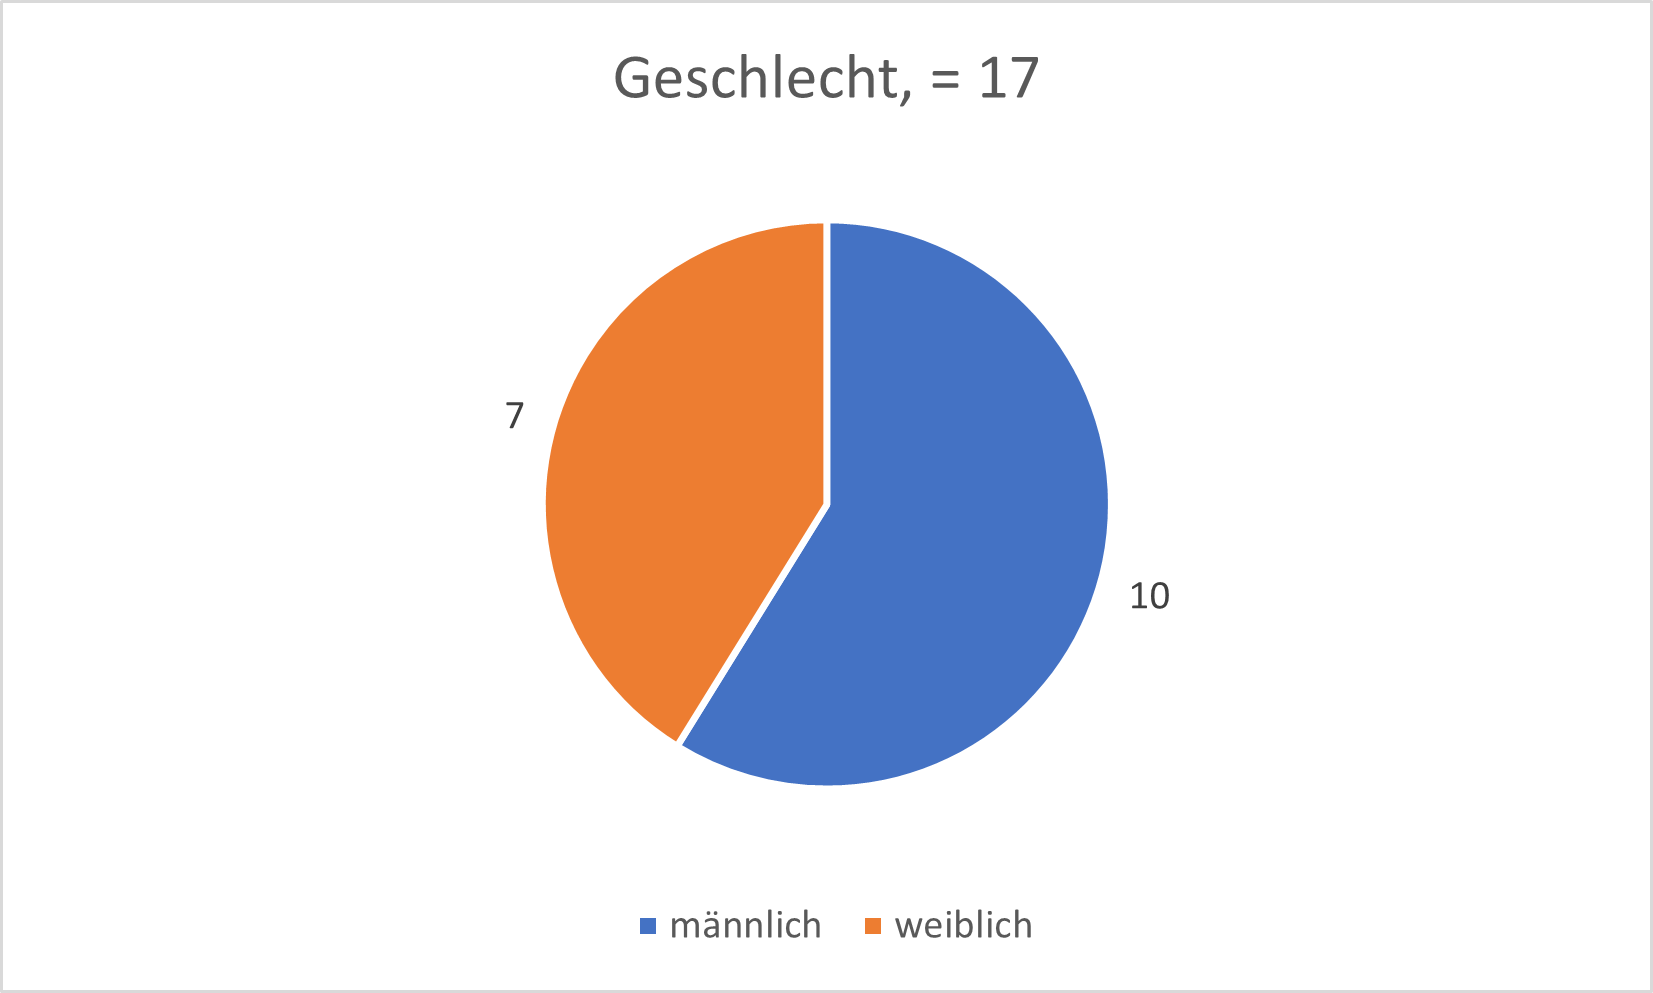
\includegraphics[width=0.2\textwidth]{assets/gesch.png} \hspace{-5pt}
	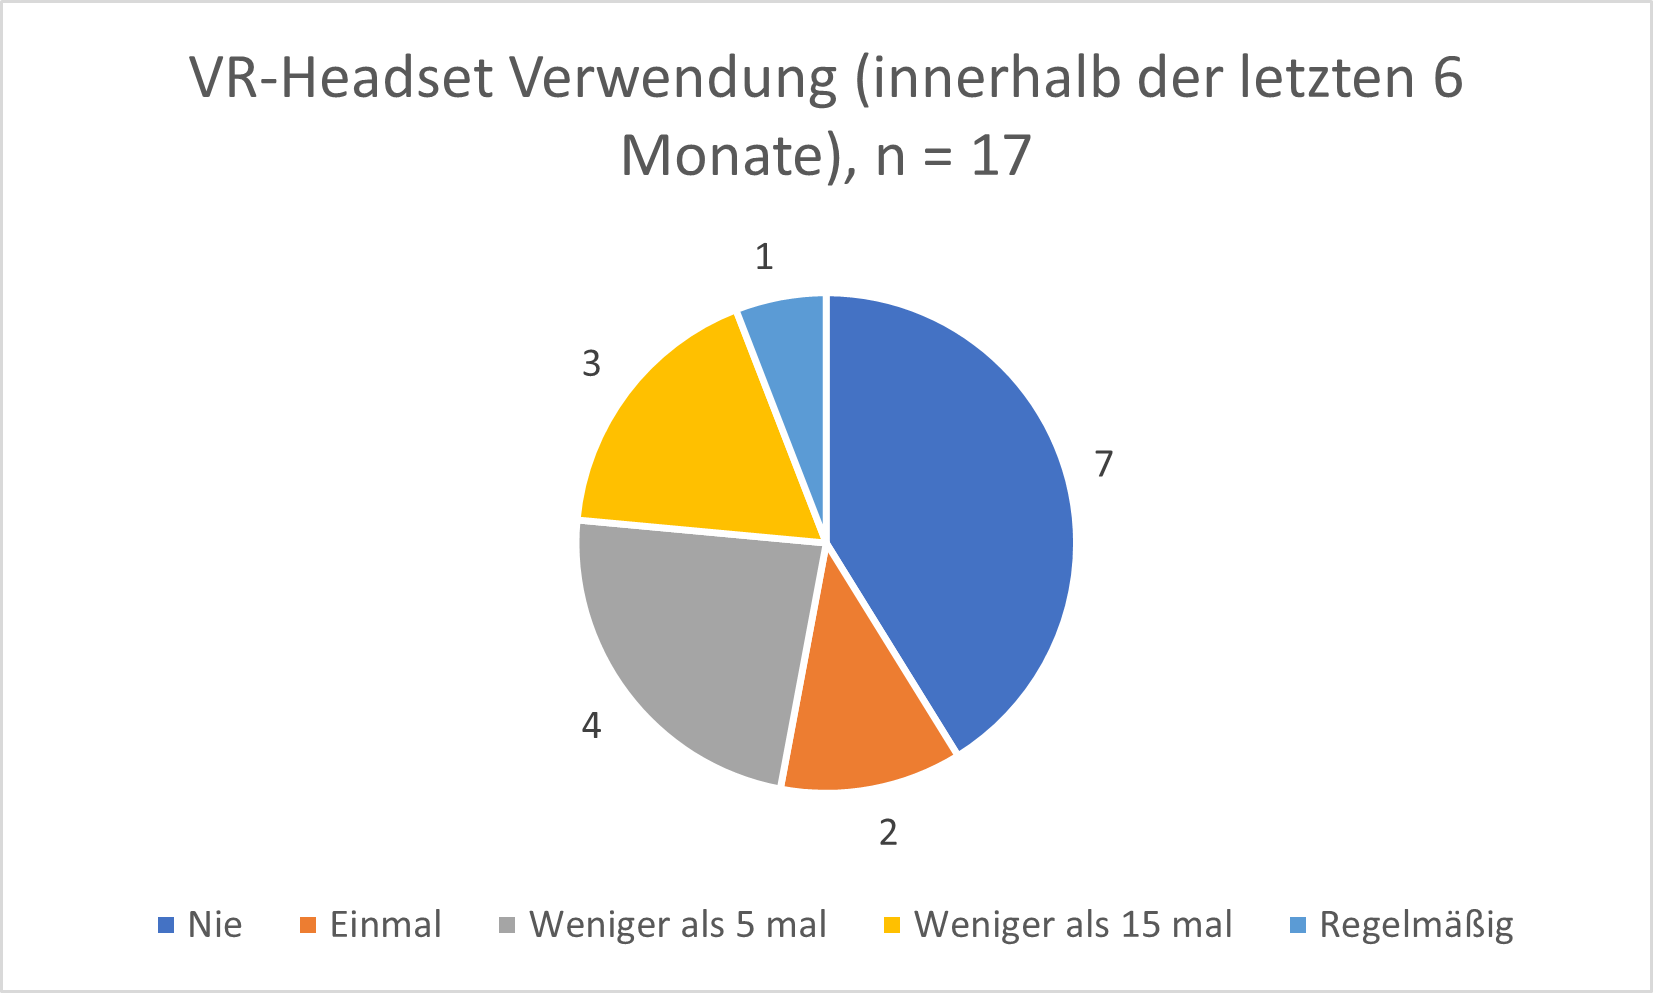
\includegraphics[width=0.2\textwidth]{assets/headset.png} \\
	\vspace{2pt}
	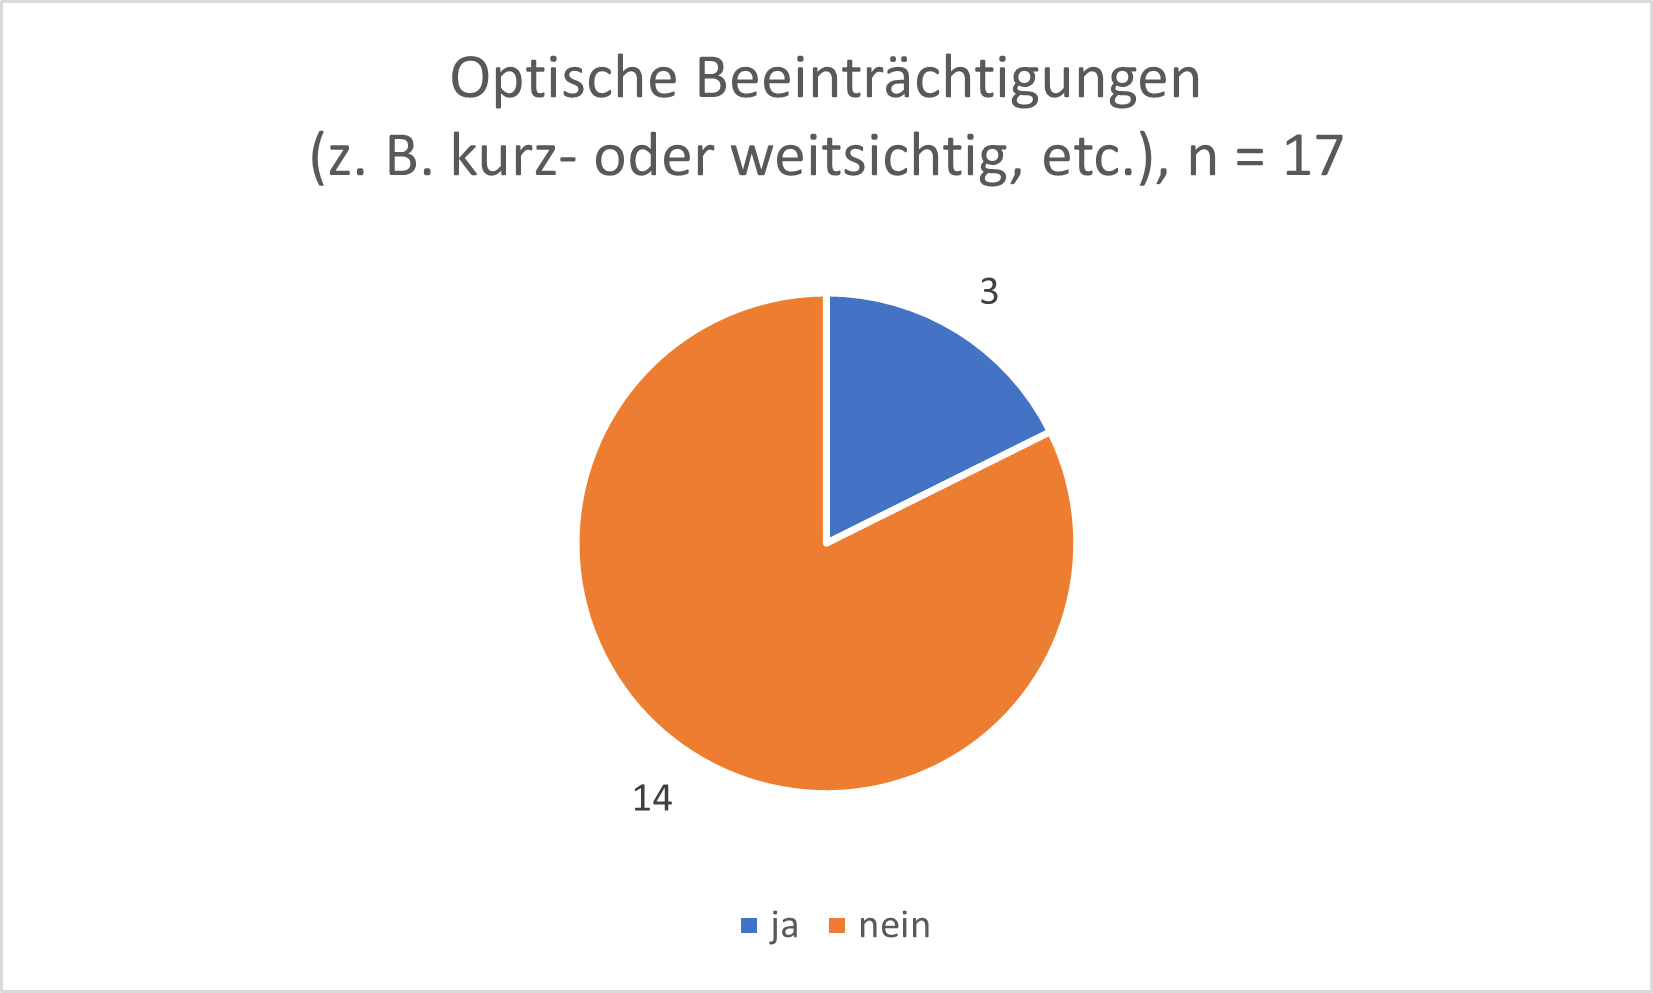
\includegraphics[width=0.2\textwidth]{assets/optBeein.png} 
	\caption{Demografische Daten 2}
	\label{fig:Demografische Daten 2}
\end{figure}
Lorem ipsum dolor sit amet, consetetur sadipscing elitr, sed diam nonumy eirmod tempor invidunt ut labore et dolore magna aliquyam erat, sed diam voluptua. At vero eos et accusam et justo duo dolores et ea rebum. Stet clita kasd gubergren, no sea takimata sanctus est Lorem ipsum dolor sit amet. Lorem ipsum dolor sit amet, consetetur sadipscing elitr, sed diam nonumy eirmod tempor invidunt ut labore et dolore magna aliquyam erat, sed diam voluptua. At vero eos et accusam et justo duo dolores et ea rebum. Stet clita kasd gubergren, no sea takimata sanctus est Lorem ipsum dolor sit amet.

\begin{figure}[ht]
	\centering
	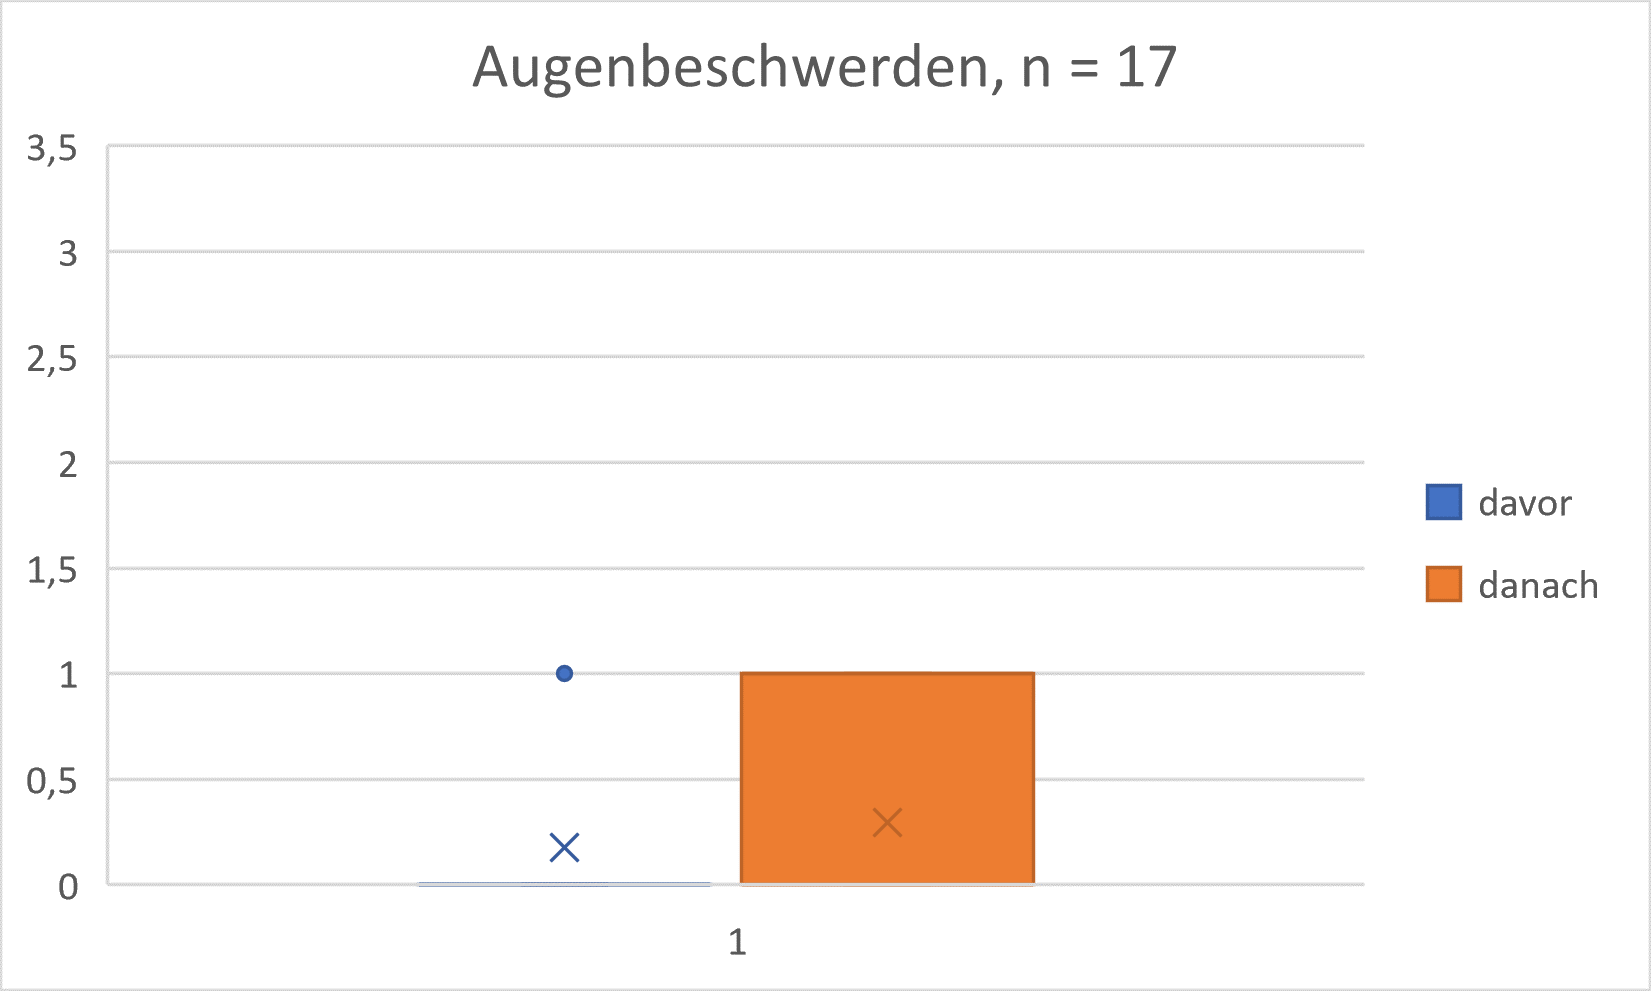
\includegraphics[width=0.2\textwidth]{assets/augenBesch.png} \hspace{-5pt}
	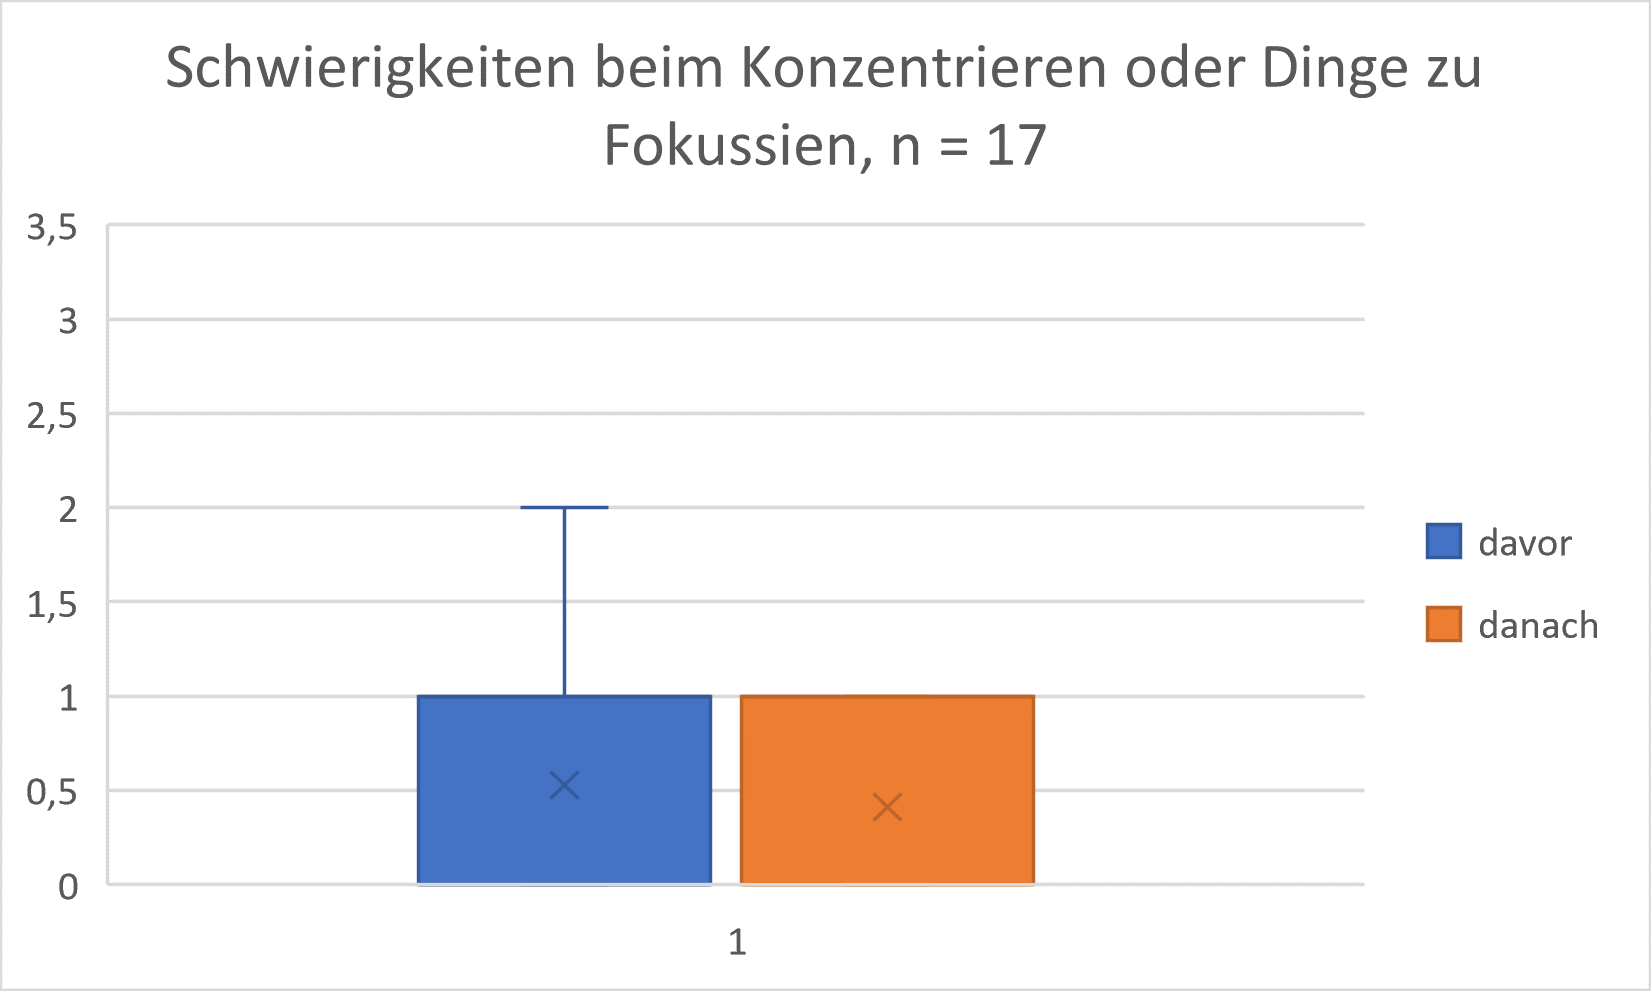
\includegraphics[width=0.2\textwidth]{assets/fokus.png} \\
	\vspace{2pt}
	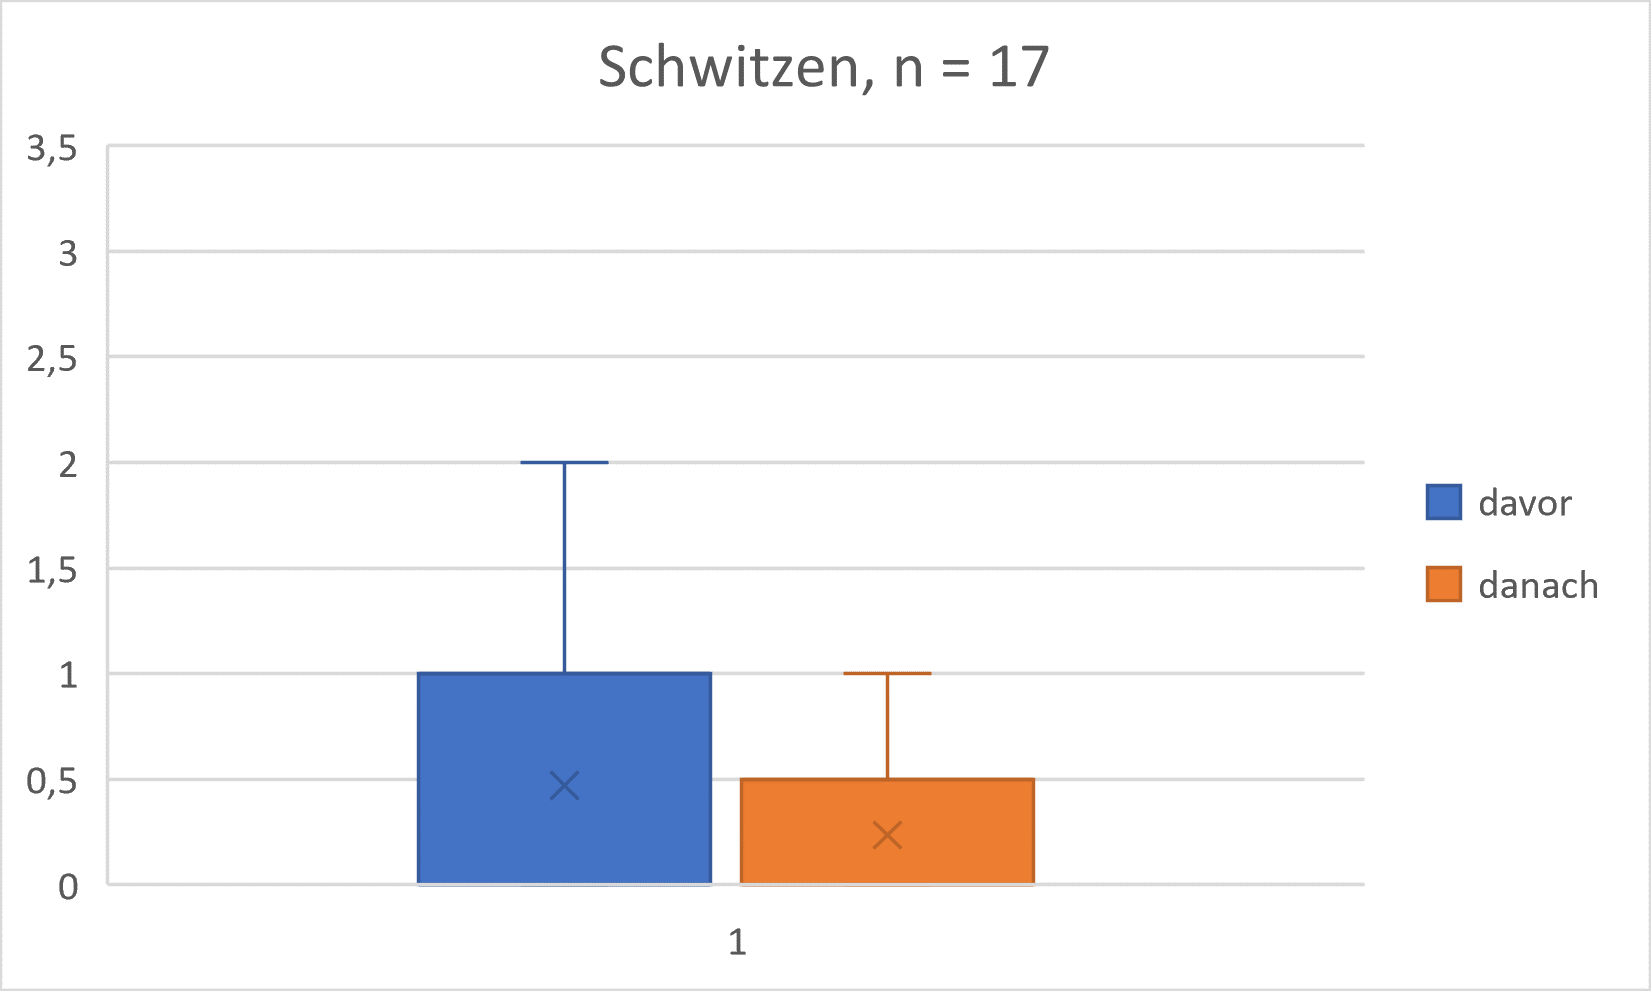
\includegraphics[width=0.2\textwidth]{assets/schwitz.png} \hspace{-5pt}
	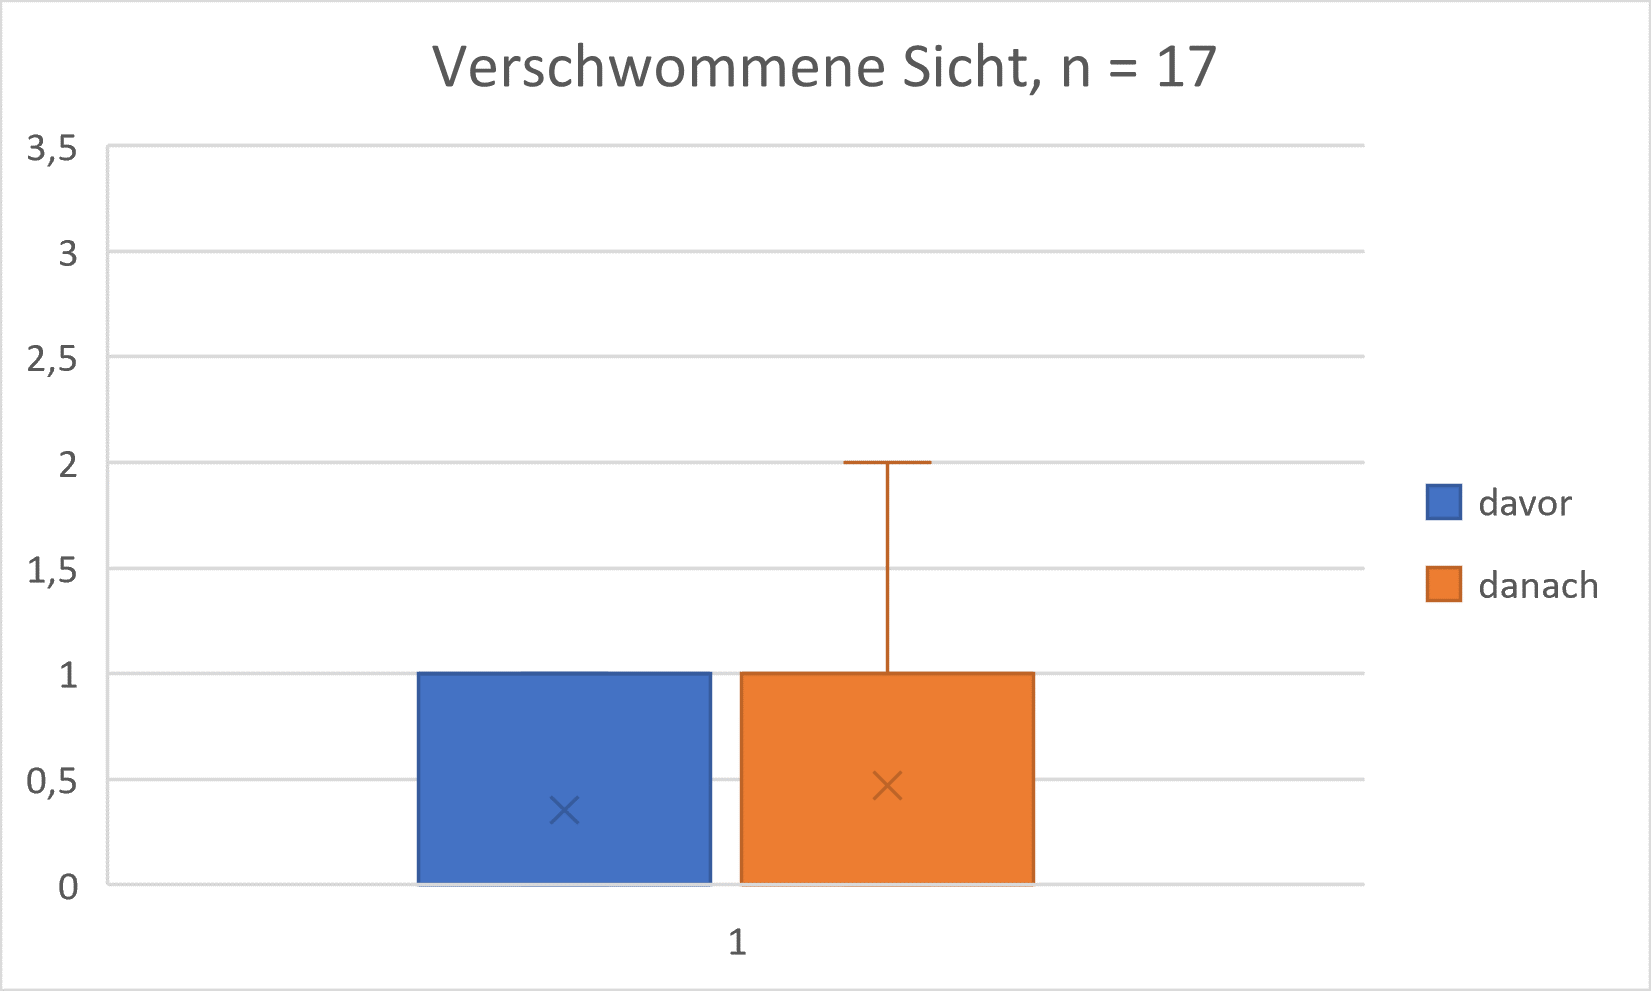
\includegraphics[width=0.2\textwidth]{assets/verschwSicht.png}
	\caption{Fragebogenergebnisse vorher nachher Vergleich}
	\label{fig:Fragebogenergebnisse}
\end{figure}
Lorem ipsum dolor sit amet, consetetur sadipscing elitr, sed diam nonumy eirmod tempor invidunt ut labore et dolore magna aliquyam erat, sed diam voluptua. At vero eos et accusam et justo duo dolores et ea rebum. Stet clita kasd gubergren, no sea takimata sanctus est Lorem ipsum dolor sit amet. Lorem ipsum dolor sit amet, consetetur sadipscing elitr, sed diam nonumy eirmod tempor invidunt ut labore et dolore magna aliquyam erat, sed diam voluptua. At vero eos et accusam et justo duo dolores et ea rebum. Stet clita kasd gubergren, no sea takimata sanctus est Lorem ipsum dolor sit amet.

Hier kommen noch mehr Ergebnisse rein...

\section{Diskussion}
Lorem ipsum dolor sit amet, consetetur sadipscing elitr, sed diam nonumy eirmod tempor invidunt ut labore et dolore magna aliquyam erat, sed diam voluptua. At vero eos et accusam et justo duo dolores et ea rebum. Stet clita kasd gubergren, no sea takimata sanctus est Lorem ipsum dolor sit amet. Lorem ipsum dolor sit amet, consetetur sadipscing elitr, sed diam nonumy eirmod tempor invidunt ut labore et dolore magna aliquyam erat, sed diam voluptua. At vero eos et accusam et justo duo dolores et ea rebum. Stet clita kasd gubergren, no sea takimata sanctus est Lorem ipsum dolor sit amet.

\section{Schlussfolgerung}
Lorem ipsum dolor sit amet, consetetur sadipscing elitr, sed diam nonumy eirmod tempor invidunt ut labore et dolore magna aliquyam erat, sed diam voluptua. At vero eos et accusam et justo duo dolores et ea rebum. Stet clita kasd gubergren, no sea takimata sanctus est Lorem ipsum dolor sit amet. Lorem ipsum dolor sit amet, consetetur sadipscing elitr, sed diam nonumy eirmod tempor invidunt ut labore et dolore magna aliquyam erat, sed diam voluptua. At vero eos et accusam et justo duo dolores et ea rebum. Stet clita kasd gubergren, no sea takimata sanctus est Lorem ipsum dolor sit amet.

\begin{thebibliography}{00}
\bibitem{b1} J. Frey, L. Pommereau, F. Lotte und M. Hachet, 'Assessing the zone of comfort in stereoscopic displays using EEG', ACM SIGCHI Conference on Human Factors in Computing Systems (S. 2041–2046. doi: 10.1145/2559206.2581191. [Online]. Verfügbar unter: https://arxiv.org/pdf/1404.6222)

\bibitem{b2} Statista. Virtual Reality - 'Prognose zum Umsatz weltweit bis 2026' | Statista. https://de.statista.com/statistik/daten/studie/318536/umfrage/prognose-zum-umsatz-mit-virtual-reality-weltweit/ (Zugriff am: 6. Juni 2023).

\bibitem{b3} A. Tatnall, Encyclopedia of education and information technologies. SPRINGER, 2020.

\bibitem{b4} U. Schmidt, Professionelle Videotechnik: Grundlagen, Filmtechnik, Fernsehtechnik (S. 27-28), Geräte- und Studiotechnik in SD, HD, DI, 3D, 6. Aufl. Berlin, Heidelberg: Springer Berlin Heidelberg; Imprint: Springer Vieweg, 2013.

\bibitem{b5} M. Guo, Y. Liu, B. Zou und Y. Wang, 'Study of electroencephalography-based objective stereoscopic visual fatigue evaluation,' in 2015 International Symposium on Bioelectronics and Bioinformatics (ISBB), 2015, S. 160–163, doi: 10.1109/ISBB.2015.7344948.

\bibitem{b6} P. Geraedts, Motorische Entwicklung und Steuerung: Eine Einführung für Physiotherapeuten, Ergotherapeuten und Trainer, 1. Aufl. Berlin, Germany: SPRINGER, 2020, S. 154-155.

\bibitem{b7} Wilder Penfield und Theodore Rasmussen, The Cerebral Cortex of Man: A Clinical Study of Localization of Function. New York: The Macmillan Company, 1950, S. 22.

\bibitem{b8} Frings, Biologie der Sinne. Springer Berlin Heidelberg, 2019, S. 193.

\bibitem{b9}Wearable Sensing | Dry EEG. DSI-24. Zugegriffen 12. Juli 2023. https://wearablesensing.com/dsi-24/.
\bibitem{b10}BESA® | Brain Electrical Source Analysis: BESA Research > Besa Research 7.1. Zugegriffen 12. Juli 2023. https://www.besa.de/home/downloads/besa-research/besa-research-7-1/.
\bibitem{b11}The professional-grade VR headset | VIVE Pro Deutschland. Zugegriffen 12. Juli 2023. https://www.vive.com/de/product/vive-pro/.


\end{thebibliography}
\vspace{12pt}
\color{red}
IEEE conference templates contain guidance text for composing and formatting conference papers. Please ensure that all template text is removed from your conference paper prior to submission to the conference. Failure to remove the template text from your paper may result in your paper not being published.

\end{document}
